% example for dissertation.sty
\documentclass[
% Replace oneside by twoside if you are printing your thesis on both sides
% of the paper, leave as is for single sided prints or for viewing on screen.
oneside,
%twoside,
11pt, a4paper,
footinclude=true,
headinclude=true,
cleardoublepage=empty
]{scrbook}

\usepackage{comment}
\usepackage{dissertation}
\usepackage{braket}
\usepackage{mathrsfs}
\newtheorem{definition}{Definition}[section]
\usepackage{mathtools}
%\usepackage{amssymb}
\usepackage{amssymb,amsmath,amsthm}
\usepackage{indentfirst} 
\usepackage{tikz}
\usepackage{physics}
%usetikzlibrary{arrows}
\DeclarePairedDelimiter\ceil{\lceil}{\rceil}
\DeclarePairedDelimiter\floor{\lfloor}{\rfloor}
\usepackage{subfiles}
\usepackage{qcircuit}
\usepackage{subcaption}
\usepackage{graphicx}
\usepackage{hyperref}
\newtheorem{post}{Postulate}

% ----------------------------------------------------------------
%University %(untomment if you need to change default values)
%\gdef\school{Escola de Engenharia}
%\gdef\department{Departamento de informática}
%\gdef\university{Universidade do Minho}
%\gdef\masterdegree{Física da informação}

% Title
%TODO: Decidir titulo.
\titleA{Quantum Random Walks}
%\titleB{Simulations and physical realizations} % (if any)
\subtitleA{Simulations and physical realizations}
%\subtitleB{Second part of Subtitle} % (if any)
\usetikzlibrary{arrows}


% Author
\author{Jaime Pereira Santos}

% Supervisor(s)
\supervisor{Luís Barbosa}
\cosupervisor{Bruno Chagas}


% Date
\date{\myear} % change to text if date is not today

% Keywords
\newcommand\englishkeywordslabel{Keywords:}
\newcommand\englishkeywords[1]{%
  \begin{list}{}{%
    \setlength{\topsep}{2ex}%
    \settowidth{\leftmargin}{\bfseries\englishkeywordslabel~}%
    \setlength{\labelsep}{0pt}%
    \setlength{\labelwidth}{\leftmargin}%
    \setlength{\itemindent}{0pt}%
  }
  \raggedright\bfseries\item[\bfseries\englishkeywordslabel~]#1
  \end{list}
}

\newcommand\portuguesekeywordslabel{Palavras-Chave:}
\newcommand\portuguesekeywords[2]{%
  \begin{list}{}{%
    \setlength{\topsep}{2ex}%
    \settowidth{\leftmargin}{\bfseries\portuguesekeywordslabel~}%
    \setlength{\labelsep}{0pt}%
    \setlength{\labelwidth}{\leftmargin}%
    \setlength{\itemindent}{0pt}%
  }
  \raggedright\bfseries\item[\bfseries\portuguesekeywordslabel~]#1
  \end{list}
}
% Glossaries & Acronyms
%\makeglossaries  %  either use this ...
%\makeindex	   % ... or this

% Define Acronyms
%%!TEX root = ../dissertation.tex

\newacronym{mei}{MEI}{Mestrado em Engenharia Inform\'{a}tica}
\newacronym{um}{UM}{Universidade do Minho}

%\glsaddall[types={\acronymtype}]


\ummetadata % add metadata to the document (author, publisher, ...)

\begin{document}
% Cover page ---------------------------------------
\umfrontcover	
\umtitlepage

\chapter*{Copyright and terms of use}
This is an academic work that can be used by third parties as long as good practices are
respected as well as internationally accepted rules concerning copyright and related rights.
Thereby, this work can be used under the terms set out in the license below.
If one needs permission to work under a different set of conditions not provided by the
indicated license, one must contact the author, through the University of Minho \textit{RepositoriUM}.
\begin{figure}[!h]
    \centering
    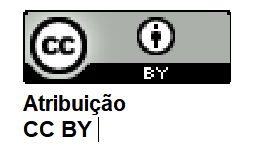
\includegraphics[scale=0.7]{img/CopyrightImg.png}
    \raggedright
\end{figure}\par
\url{https://creativecommons.org/licenses/by/4.0/}

\chapter*{STATEMENT OF INTEGRITY}
I hereby declare having conducted this academic work with integrity. I confirm that I have not used plagiarism or any form of undue use of information or falsification of results along the process leading to its elaboration. 
I further declare that I have fully acknowledged the Code of Ethical Conduct of the University of Minho.

% Add acknowledgements ----------------------------
\chapter*{Acknowledgements}
\subfile{Chapters/Abstract/acknowledgements}

% Add abstracts (en,pt) ---------------------------
\chapter*{Abstract}
\subfile{Chapters/Abstract/abstract}
\englishkeywords{Quantum Computing\quad Quantum Walks\quad Python \quad Qiskit}



\cleardoublepage
\chapter*{Resumo}
\subfile{Chapters/Abstract/resumo}
\portuguesekeywords{Computação Quântica\quad Caminhadas Quânticas\quad Python\quad Qiskit}

% Summary Lists ------------------------------------
\tableofcontents
\listoffigures
\listoftables
%\lstlistoflistings
%\listofabbreviations


\pagenumbering{arabic}

% CHAPTER - Introduction -------------------------
\chapter{Introduction}\label{chap:introduction}
\subfile{Chapters/Chapter1/chapter1intro}
\section{Brief History of Quantum Computing}\label{sec:historyQC}
\subfile{Chapters/Chapter1/historyQC}
\section{Classical and Quantum Walks}\label{sec:classicalandquantumwalks}
\subfile{Chapters/Chapter1/randomWalks}
\section{State of the Art on Quantum Walk Implementations}\label{sec:stateart}
\subfile{Chapters/Chapter1/stateArtQW}
\section{Objectives, Contributions and Structure}\label{sec:contrib}
\subfile{Chapters/Chapter1/txtoverview}

% CHAPTER - Quantum Walks. -------------------------
\chapter{Quantum Walks}\label{chap:QuantumWalks}
\subfile{Chapters/Chapter2/chapter2intro}
\section{Classical Random Walk}\label{sec:chap3ClassicalWalk}
\subfile{Chapters/Chapter2/classicalWalk}
\section{Coined Quantum Walk}\label{sec:chap3Coinedwalk}
\subfile{Chapters/Chapter2/coinedQuantumWalk}
\section{Staggered Quantum Walk}\label{sec:chap3StagWalk}
\subfile{Chapters/Chapter2/staggeredQuantumWalk}
\section{Continuous-Time Quantum Walk}\label{sec:chap3Contwalk}
\subfile{Chapters/Chapter2/continuousQuantumWalk}


% CHAPTER - Searching Problems. -------------------------
\chapter{Searching Problems}\label{chap:searchingProblems}
\subfile{Chapters/Chapter3/chapter3intro}
\section{Grover's Algorithm}\label{sec:GrovSearchSimul}
\subfile{Chapters/Chapter3/groverAlgorithm}
\section{Coined Quantum Walk}\label{sec:CoinedSearchSimul}
\subfile{Chapters/Chapter3/coinedSearch}
\section{Staggered Quantum Walk}\label{sec:StagSearchSimul}
\subfile{Chapters/Chapter3/stagSearch}
\section{Continuous-Time Quantum Walk}\label{sec:ContSearchSimul}
\subfile{Chapters/Chapter3/contSearch}


% CHAPTER - Qiskit Implementations. -------------------------
\chapter{Implementations and Applications}\label{chap:qiskitImplementation}
\subfile{Chapters/Chapter4/chapter4Intro}
\section{Coined Quantum Walk}\label{sec:CoinedQiskit}
\subfile{Chapters/Chapter4/coinedQWQiskit}
\section{Staggered Quantum Walk}\label{sec:StagQiskit}
\subfile{Chapters/Chapter4/stagQWQiskit}
\section{Continuous-Time Quantum Walk}\label{sec:ContQiskit}
\subfile{Chapters/Chapter4/contQWQiskit}
\section{Implementing Search Algorithms in Qiskit}\label{sec:SearchProblemsQiskit}
\subfile{Chapters/Chapter4/searchProblemsQiskit}

% CHAPTER - Conclusion/Future Work -------------- 
\chapter{Discussions and Conclusion}
%\section{Conclusions}
\subfile{Chapters/Chapter5/Conclusions}

\bookmarksetup{startatroot} % Ends last part.
\addtocontents{toc}{\bigskip} % Making the table of contents look good.
%\cleardoublepage

%- Bibliography (needs bibtex) -%
\bibliography{bibliography}

% Index of terms (needs  makeindex) -------------
%\printindex


% APPENDIX --------------------------------------
\umappendix{Appendix}

% Add appendix chapters
\chapter{Support Material}
\section{The Postulates of Quantum Mechanics}\label{sec:PostulatesQM}
\subfile{Chapters/Annex/MathematicalFoundations/postulatesQM}
\section{Quantum Fourier Transform}\label{sec:chapQFT}
\subfile{Chapters/Annex/Circuits/qFourierT}

% \chapter{Mathematical Foundations}
% \section{The Postulates of Quantum Mechanics}\label{sec:PostulatesQM}
% \subfile{Chapters/Annex/MathematicalFoundations/postulatesQM}
% \chapter{Some Useful Circuits}
% \section{Quantum Fourier Transform}\label{sec:chapQFT}
% \subfile{Chapters/Annex/Circuits/qFourierT}
% \section{Diagonal Function}
% \subfile{Chapters/Annex/Circuits/diagonal}

%	\umbackcover{
%	NB: place here information about funding, FCT project, etc in which the work is %framed. Leave empty otherwise.
%	}


\end{document}
